\section{RESULTS}

Both 1D and 2D simulations across a wide range of parameters have been successfully performed. In figure \ref{fig:single_bounce} a single bounce of $\psi$ across a strong barrier can be seen (1D). The wave function drops onto the barrier, is reflected upward, then drops again due to gravity. This process continues. The transmitted component is absorbed by the CAP and can be clearly seen in the image. Multiple bounces can be seen in figure \ref{fig:many_bounces} and a long-term run with a strong barrier can be seen in figure \ref{fig:long-term-run} on page \pageref{fig:long-term-run}. Calculated arrival time distributions across different barrier strengths can be seen in figure \ref{fig:arrival_time_freefall_diff_gammas} on page \pageref{fig:arrival_time_freefall_diff_gammas}, giving a clear representation of "arrival time peaks" at the detector.

\begin{figure}
    \centering
    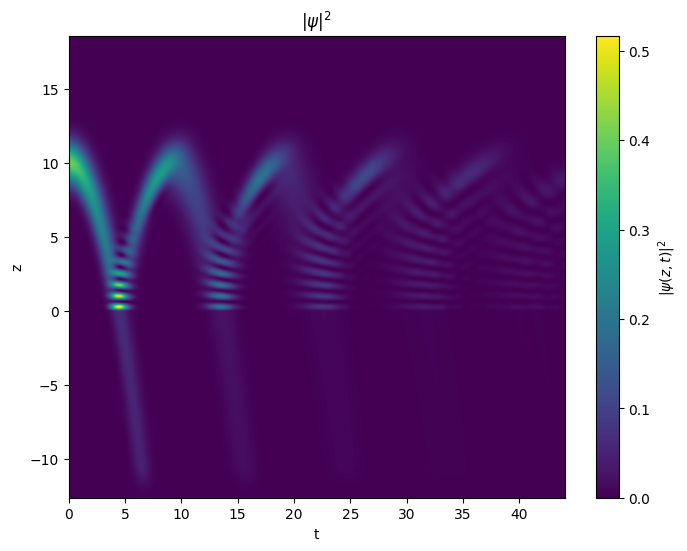
\includegraphics[width=1\linewidth]{Figures//1d_arrival_time/many_bounces.png}
    
    \caption{Showing $|\psi|^2$ of a  quantum particle falling under free fall, the transmitted component is absorbed at the boundary of the simulation. The reflected part of the wave function falls back down to the barrier. A detector is placed at $z=-L=-5$}
    \label{fig:many_bounces}
\end{figure}

\subsection{$\bigO(dt^3)$ vs $\bigO(dt^5)$ Simulations}

A few experiments across a wide range of parameters have been conducted to assess the difference in predicted arrival time distributions. Even for long runs (100+ s), the difference between the arrival time distributions doesn't exceed $1.75 \times 10^{-8}$ in probability per unit time (PPT), on average, across the considered time domain. The first arrival time peak is impacted with the biggest error, hence the difference in first peak between both methods across a wide range of drop heights and barrier strengths has been conducted, whose results can be seen in the heatmap in figure \ref{fig:difference_wide_parameters}, an explicit difference plot between both methods can be found in the appendix.

\begin{figure}
    \centering
    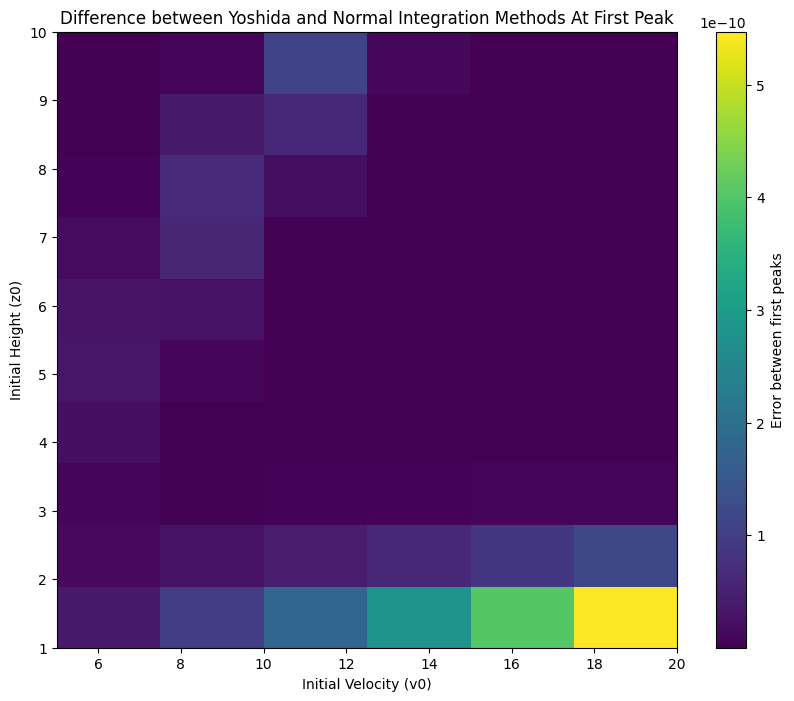
\includegraphics[width=1\linewidth]{Figures//Yoshida/70d7857a-0990-4979-969a-5731ac2add2b.png}
    \caption{First Peak Difference in Arrival Time Density Between $\bigO(dt^3)$ and $\bigO(dt^5)$ methods}
\label{fig:difference_wide_parameters}
\end{figure}

The first peak error doesn't exceed more than $5 \times 10^{-10}$ PPT, but given the sensitive nature of the analysis, all 1D simulations have been conducted with \textbf{Yoshida's method} for its improved accuracy.

\subsection{Arrival Time Distributions}

Delta-type and Gaussian-type Arrival Time distributions are run for different simulation parameters. The delta-type barriers seem to give classic-like arrival time distributions for different barrier strengths heights (figure \ref{fig:arrival_time_freefall_diff_gammas} on page \pageref{fig:arrival_time_freefall_diff_gammas}). Arrival times for Gaussian barriers clearly show \textit{non-trivial} arrival time distributions.
\\\\
This is most clearly noticeable by plotting the \textbf{arrival time distribution peaks}, focusing on their temporal distribution and intensity distribution across changing parameters, like barrier strength, and drop height. The main results can are compiled in figures \ref{fig:peak_barrier_vs_secs} with more available in the appendix starting from page \pageref{fig:particle_drop_height_power}, including isolated cases for closer inspection of the intricate non-linear results.

% \begin{figure}
%     \centering
%     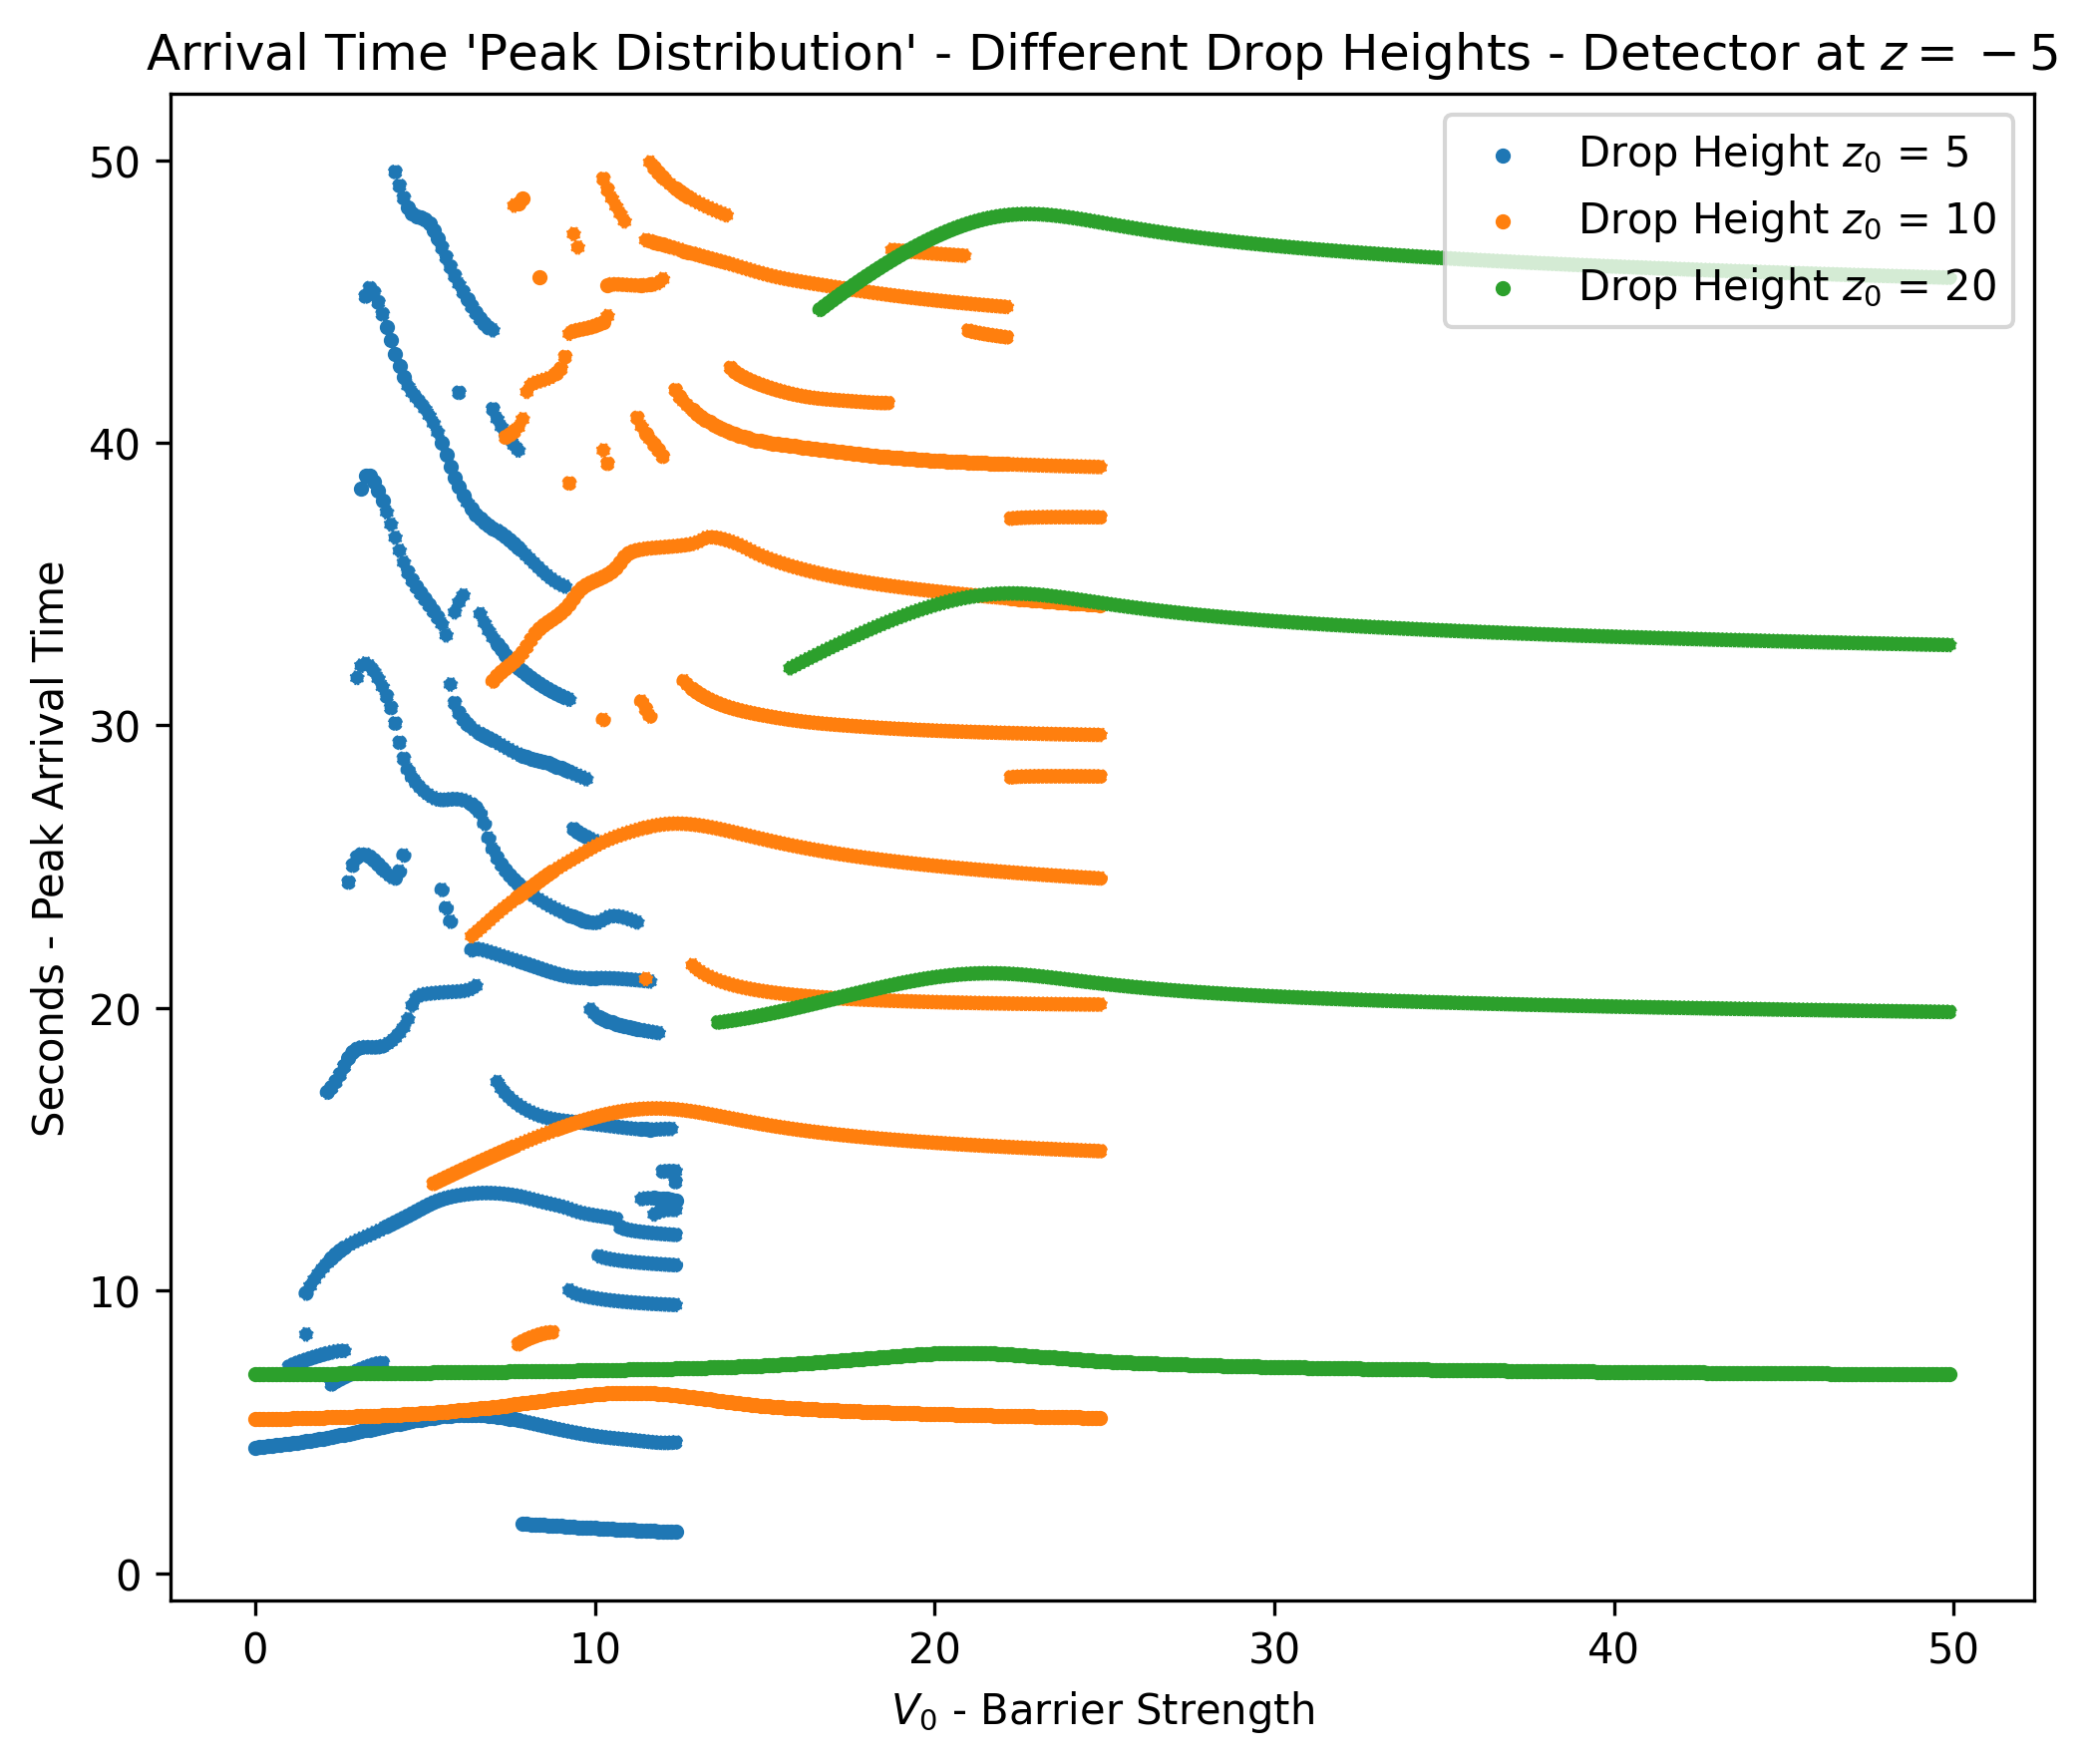
\includegraphics[width=1\linewidth]{Figures//Yoshida/6663e0ce-fb89-4819-b390-3bad6ba0e3c4.png}
%     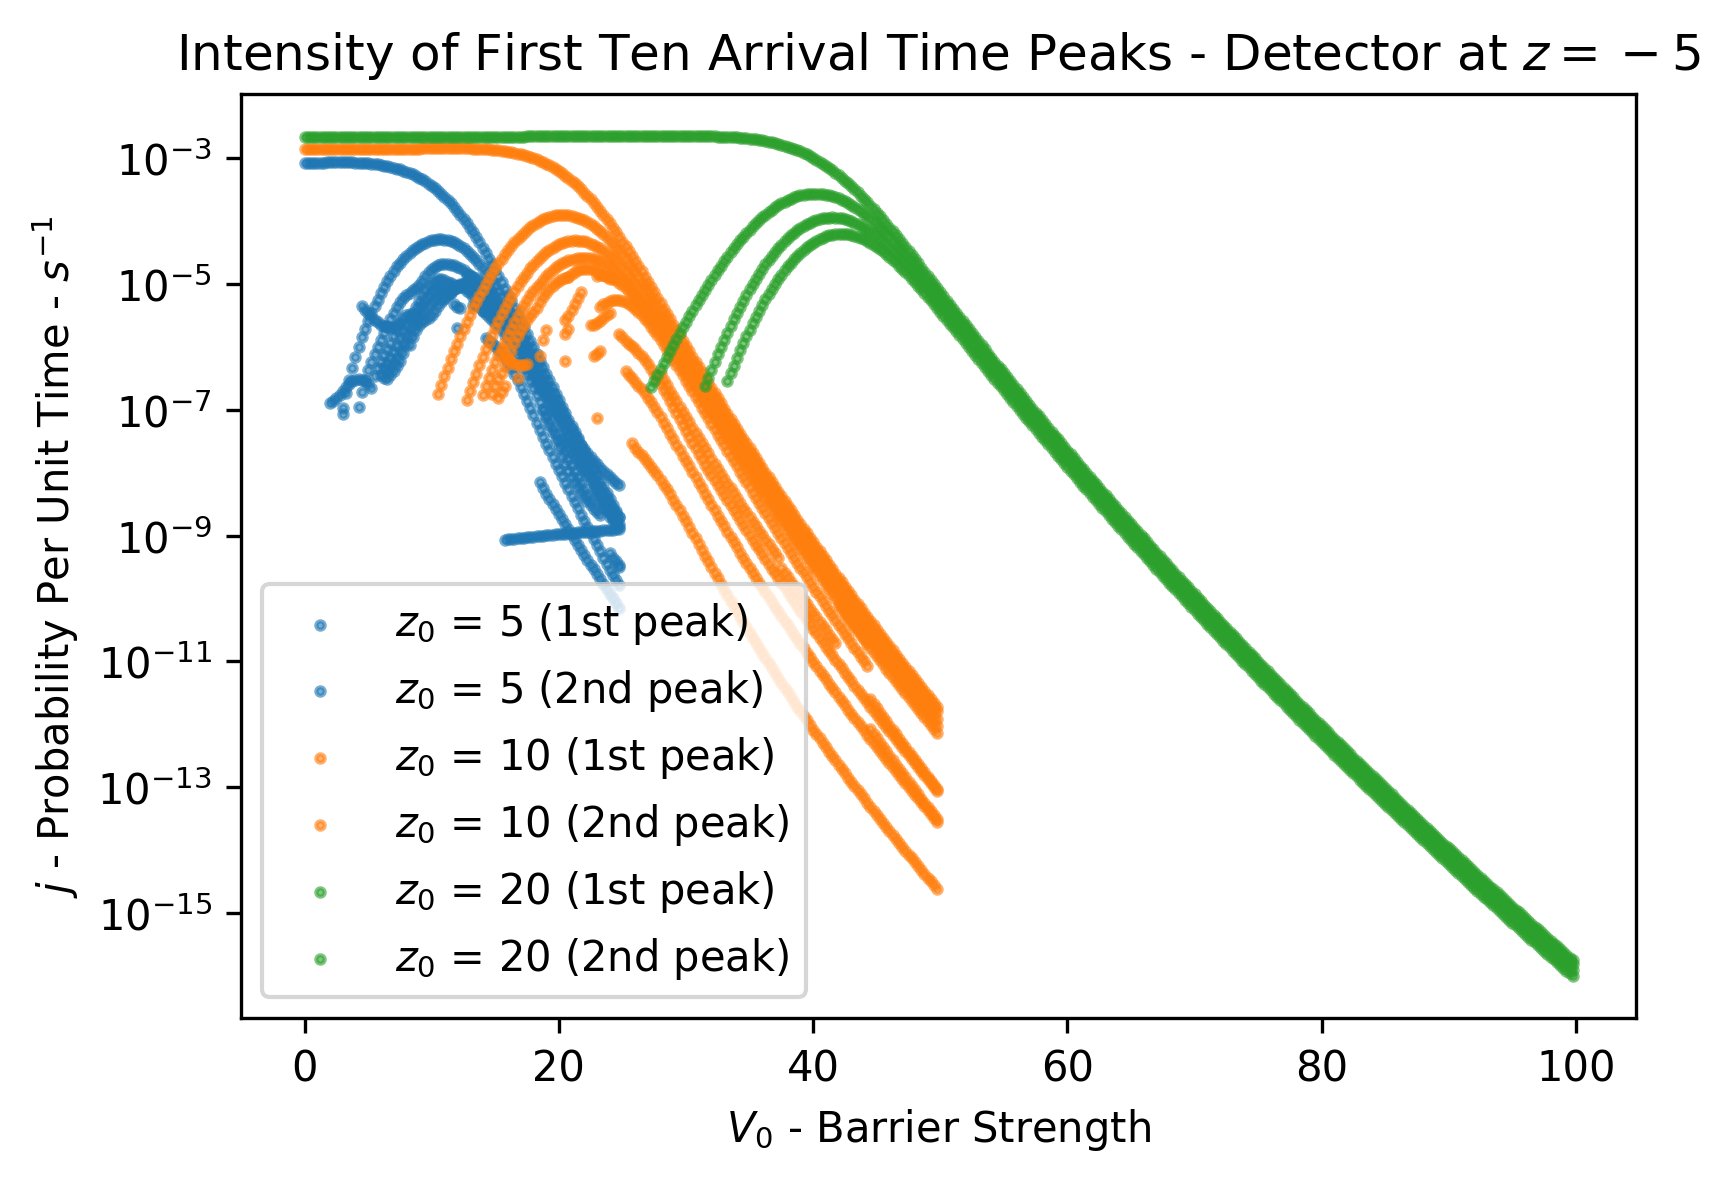
\includegraphics[width=1\linewidth]{Figures//Yoshida/2897f6b7-dd93-43e5-8846-e3fb0f150b28.png}
%     \caption{First Peak Difference in Arrival Time Density Between $\bigO(dt^3)$ and $\bigO(dt^5)$ methods}
%     \label{fig:peak_barrier_vs_secs}
% \end{figure}

\begin{figure}
    \centering
    \begin{subfigure}[b]{1\linewidth}
        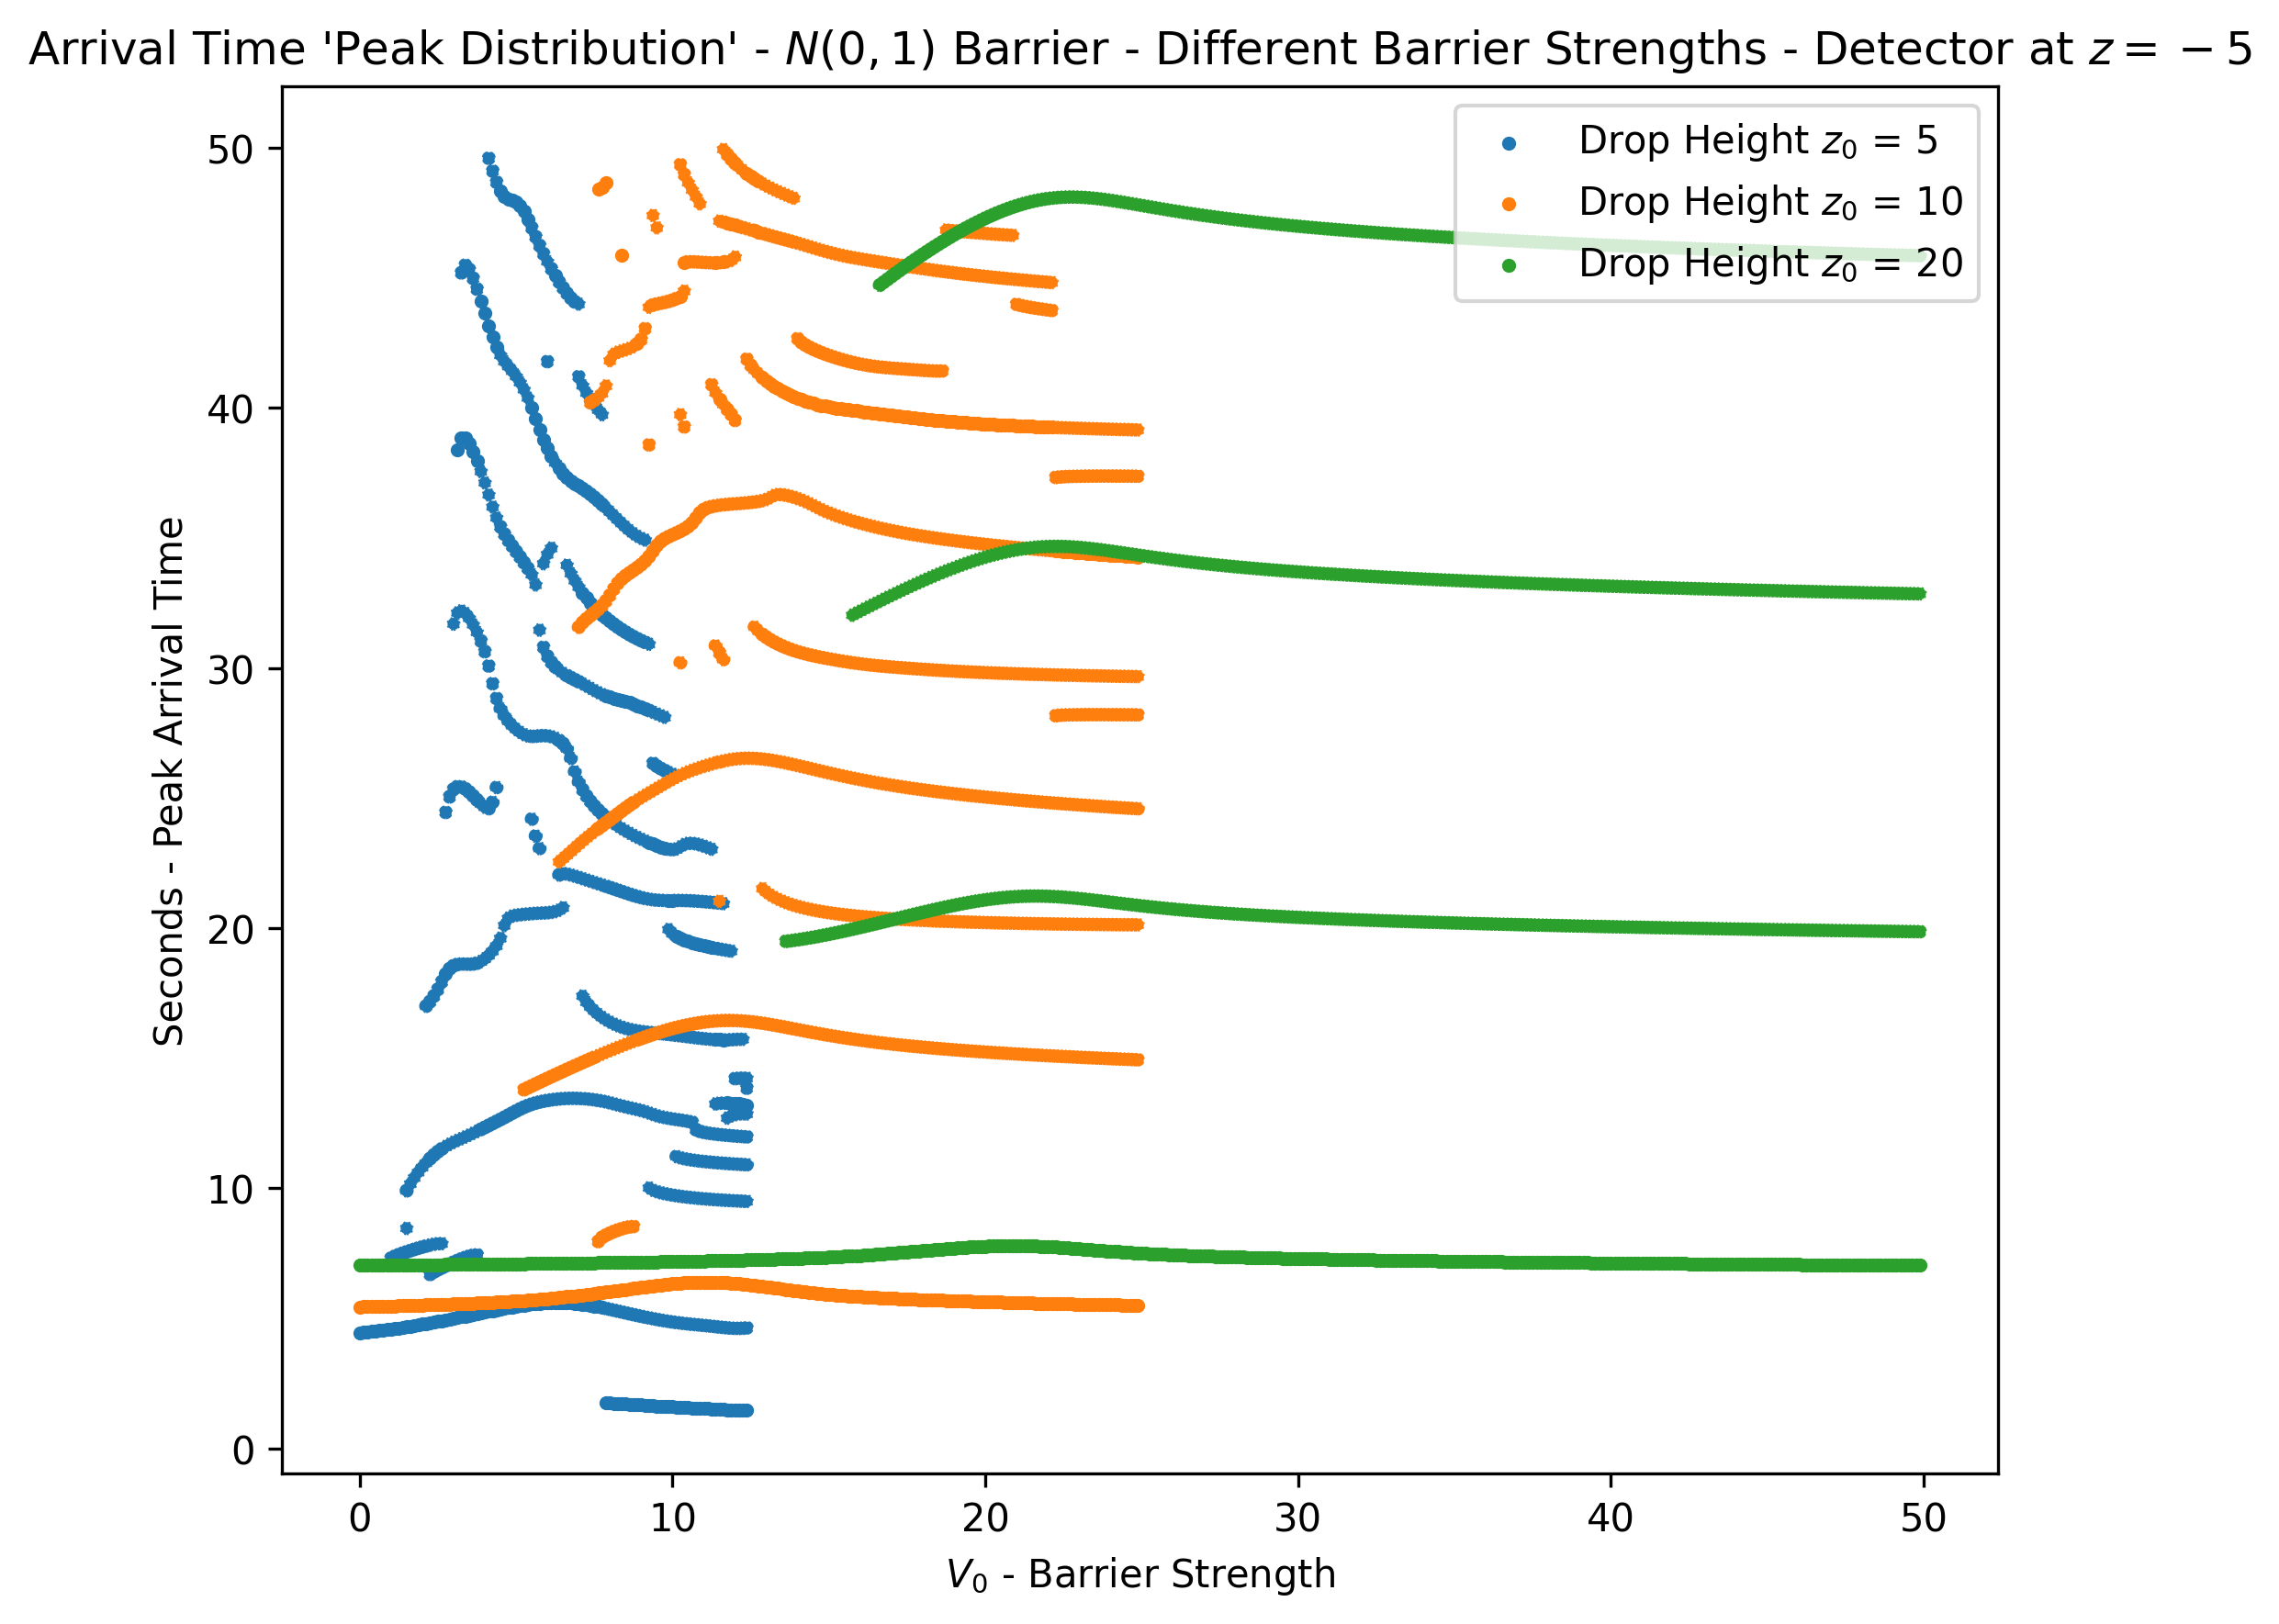
\includegraphics[width=\linewidth]{Figures//Yoshida/3444d7de-b27d-4a56-9831-5486c5e74929.png}
        \caption{}
    \end{subfigure}
    \\
    \begin{subfigure}[b]{1\linewidth}
        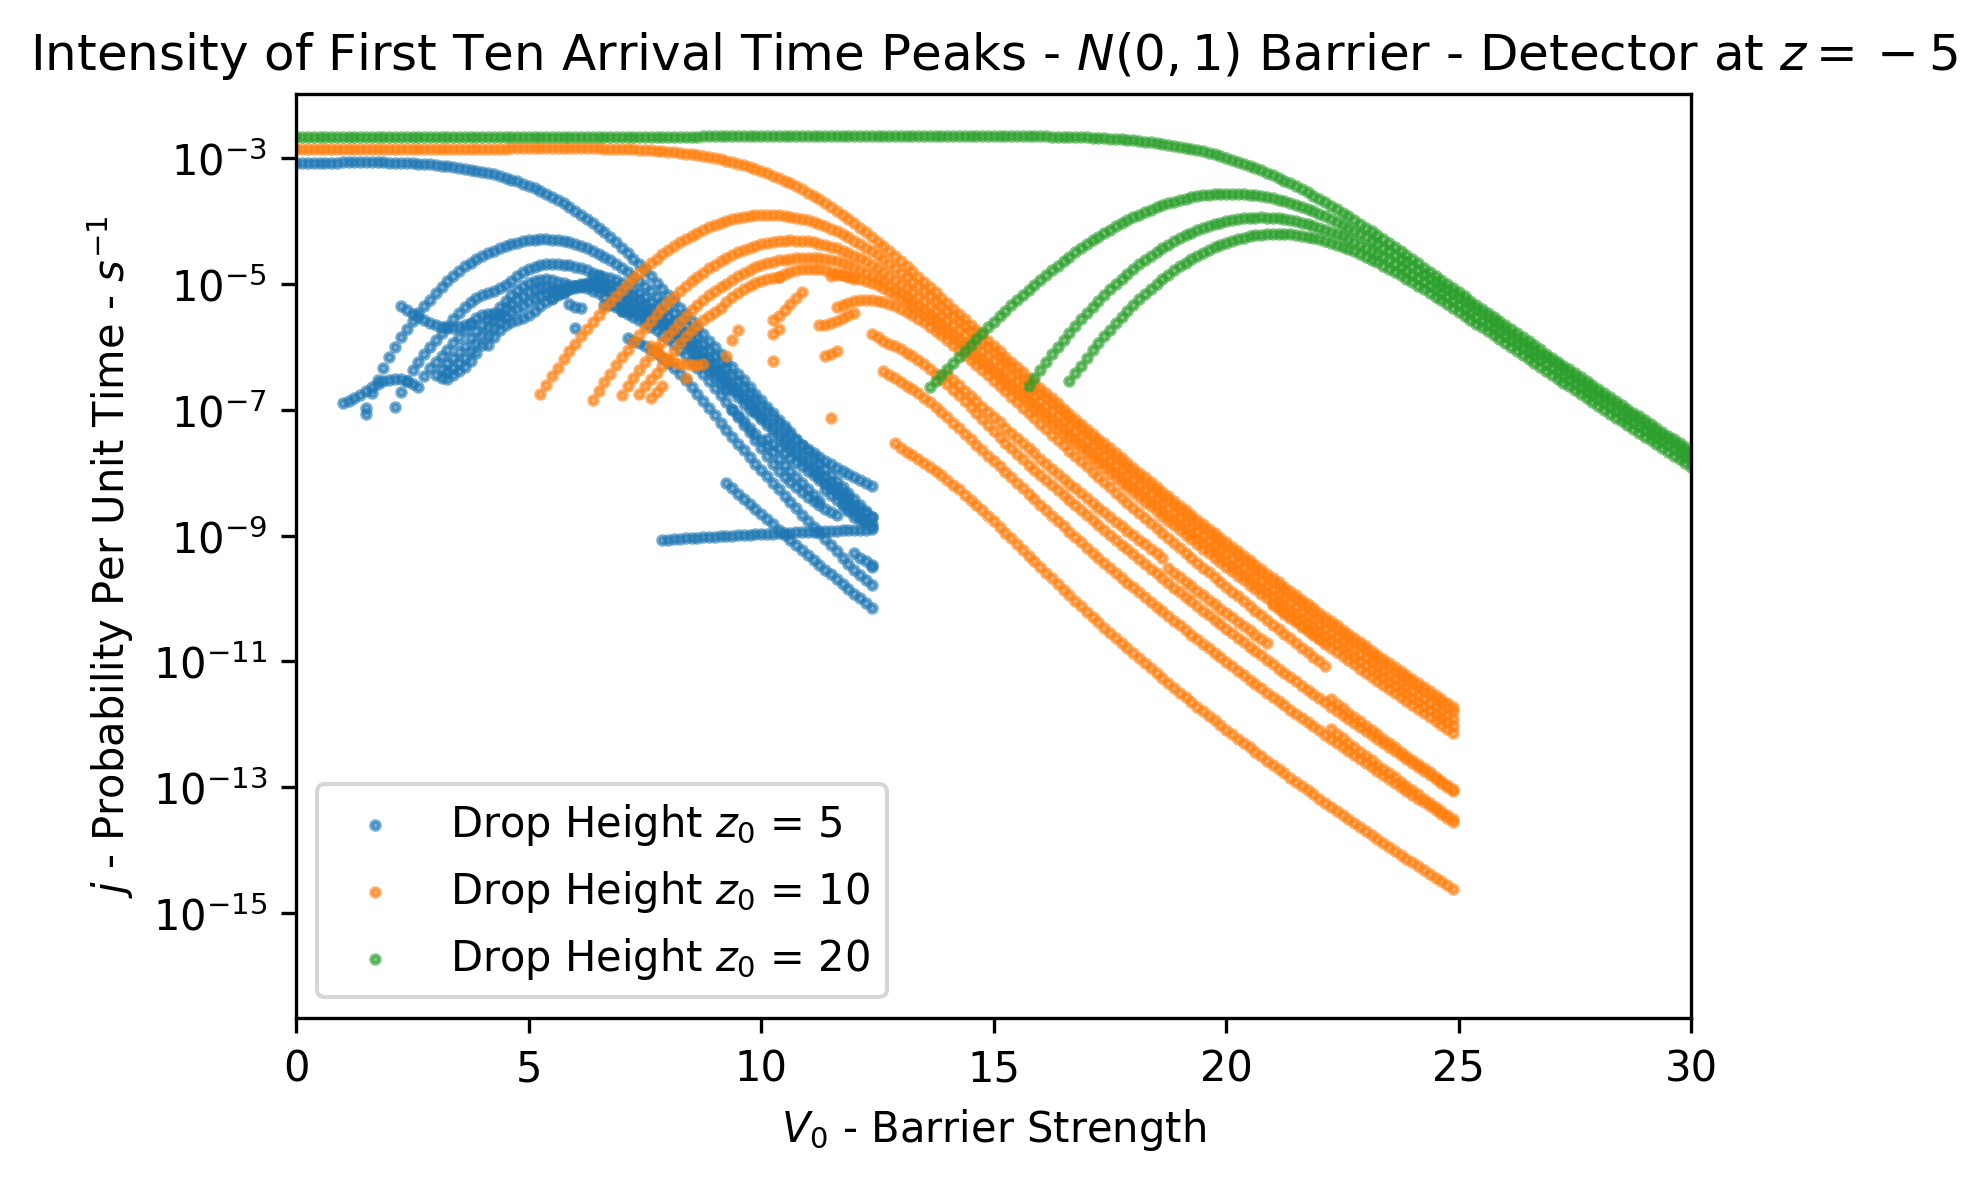
\includegraphics[width=\linewidth]{Figures//Yoshida/e3ca365e-0e36-49bf-87a0-363c8a26e34f.png}
        \caption{}
    \end{subfigure}
    \\
    \begin{subfigure}[b]{1\linewidth}
        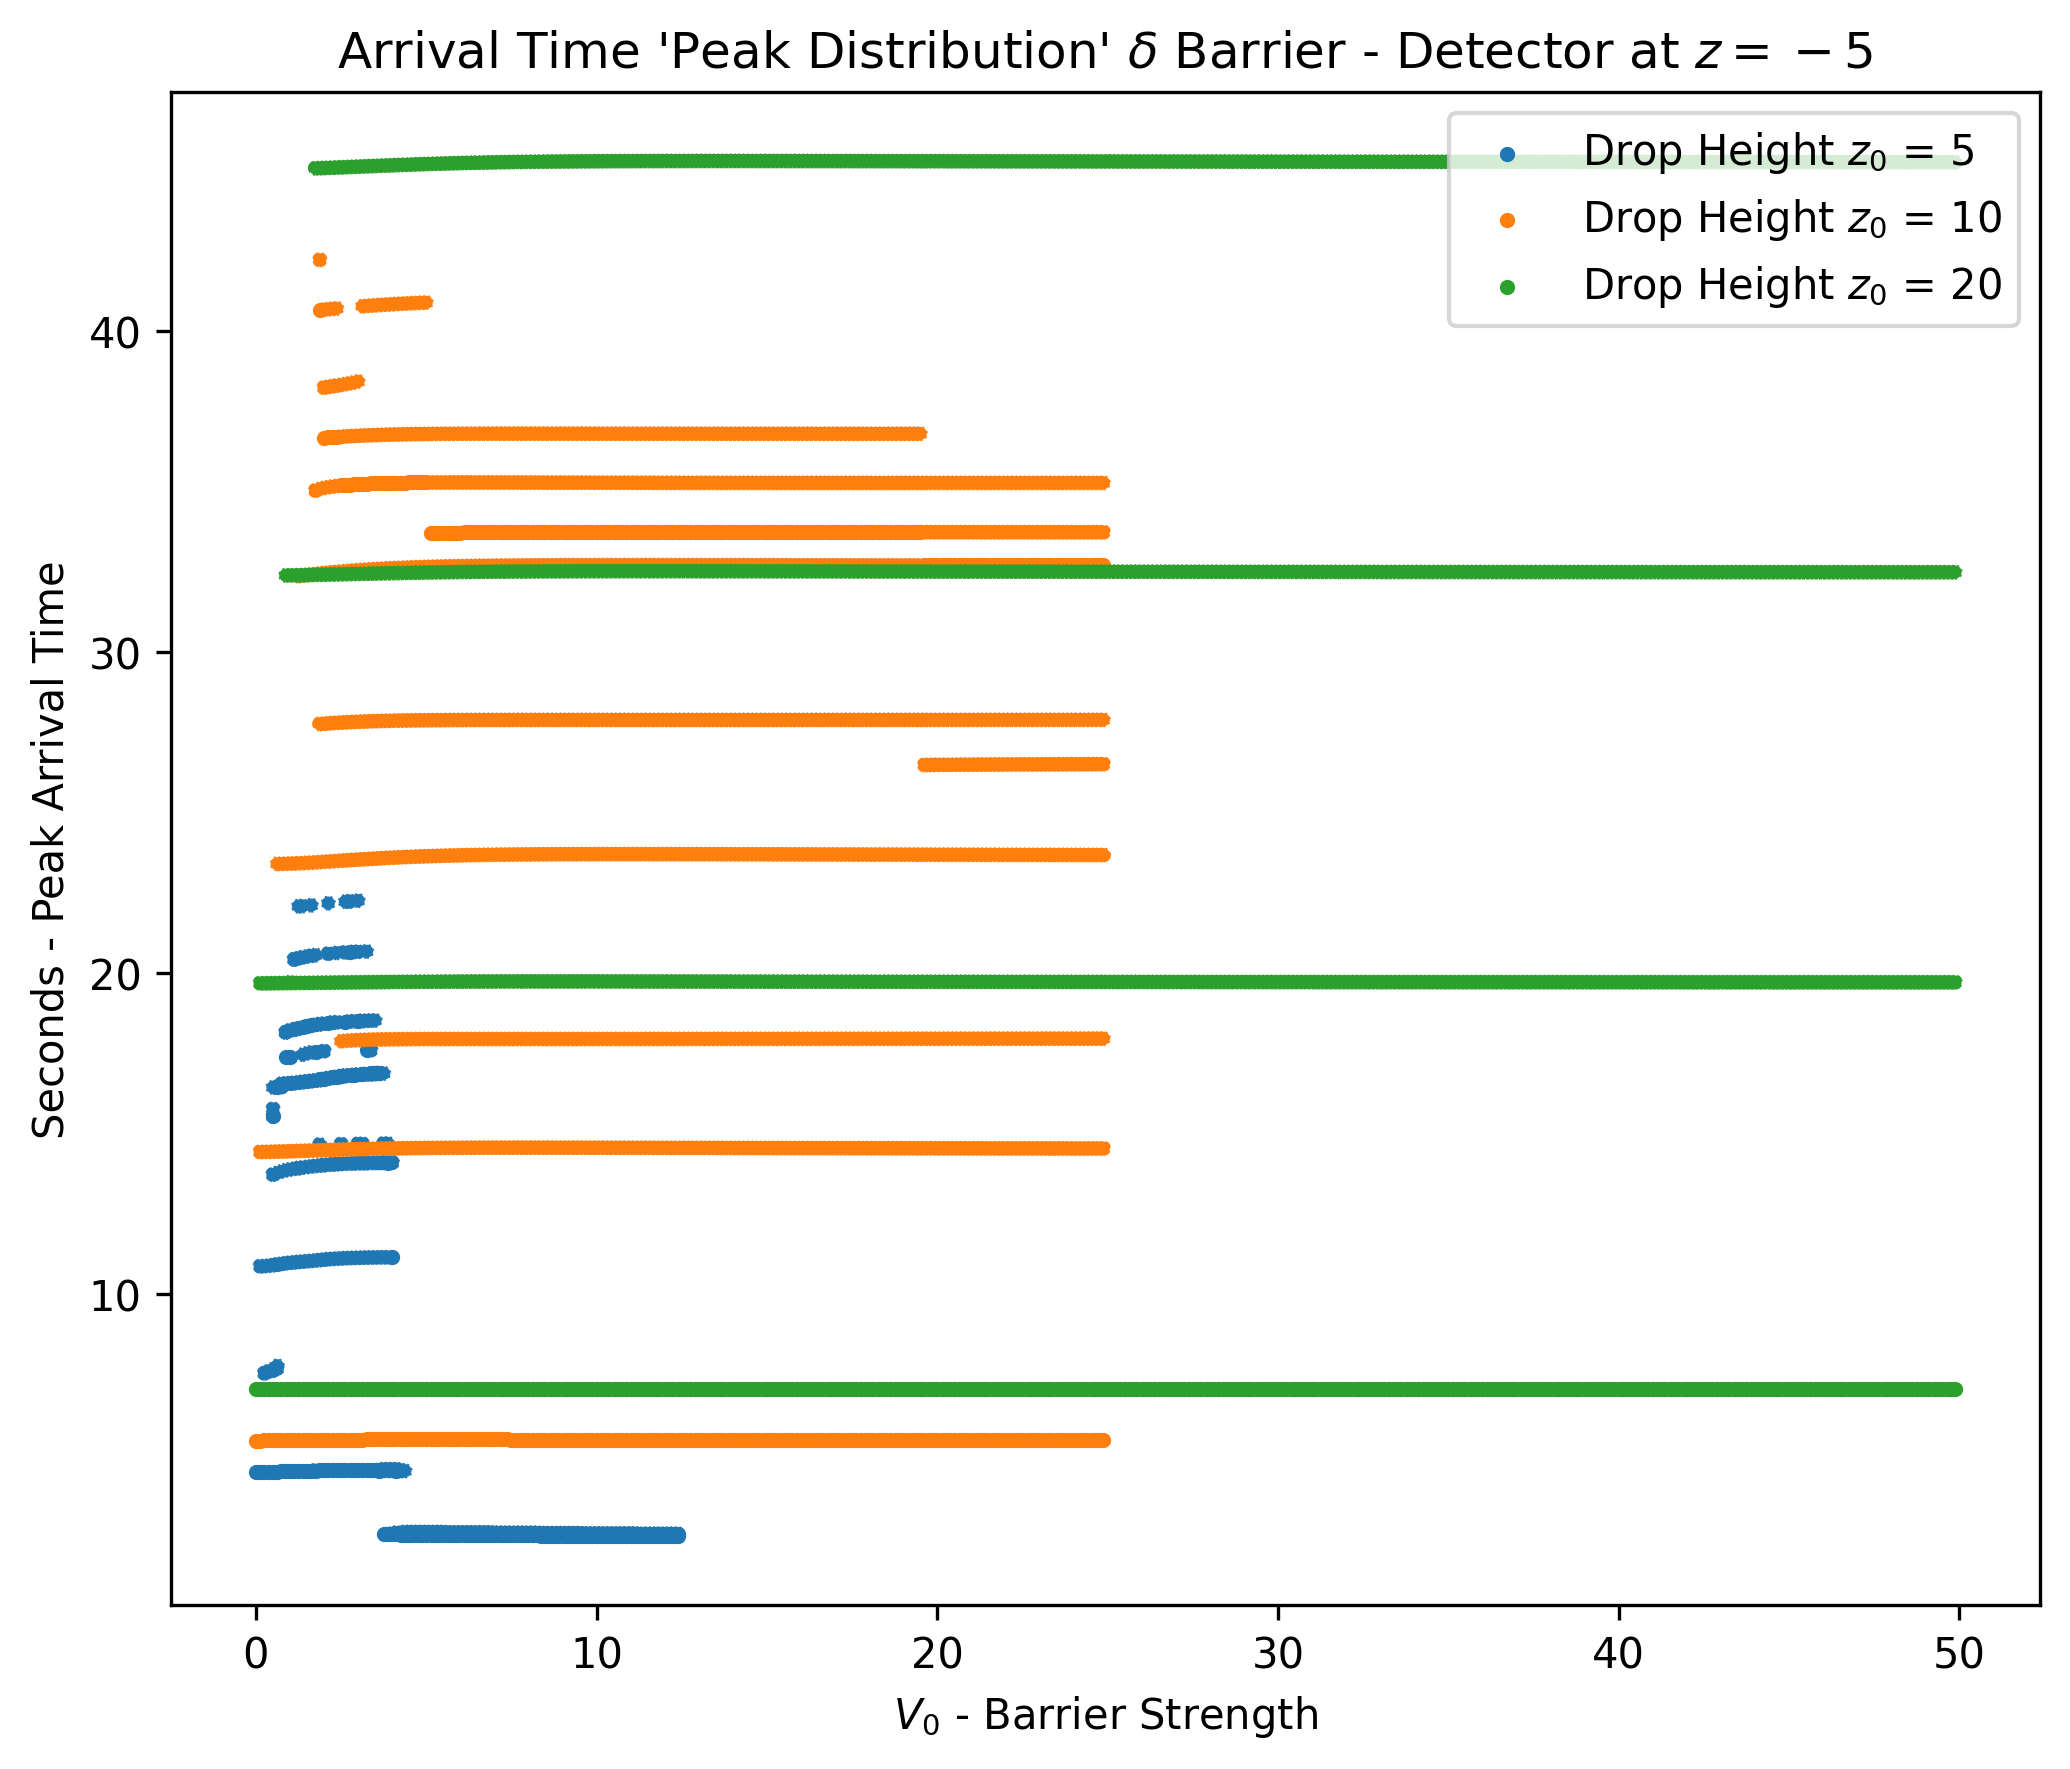
\includegraphics[width=1\linewidth]{Figures//Yoshida/7d42f617-724e-4ce1-9783-f4b1483645be.png}
        \caption{}
    \end{subfigure}
    \caption{Arrival Time Distribution Peak \textbf{times (a)} and their corresponding \textbf{intensities (b)} are plotted in function of barrier strength $V_0$: the dots in each vertical slice represent the peaks of the arrival time distribution. \textbf{(c)} represents arrival time peaks for a \textbf{delta barrier}.}
    \label{fig:peak_barrier_vs_secs}
\end{figure}

\subsection{Fitting Peaks}

An interesting feature of the produced arrival time distributions is that their \textbf{peaks} look as if they are exponentially decaying over time. An attempt has been made to characterize the \textbf{decay constant $\lambda$} of these peaks. A clear linear correlation can be witnessed when plotting the arrival time peaks and its corresponding fit, on a logarithmic scale, as can be seen in on top in figure \ref{fig:peak_barrier_vs_j}. The retrieved reciprocal value for $\tau = \frac{1}{\lambda}$ are plotted for various drop heights $z_0$ and barrier strengths $V_0$ in figure \ref{fig:peak_barrier_vs_j}, which includes error bars that represent 3000 $\times$ the mean square error of the fit against the peaks. At least three peaks had to be identified for a fit to proceed, and peaks were identified as being local maxima, with intensities of at least $0.0001\%$ of the first peak's PPT value (consistently the maximum intensity).

\begin{figure}
    \centering
    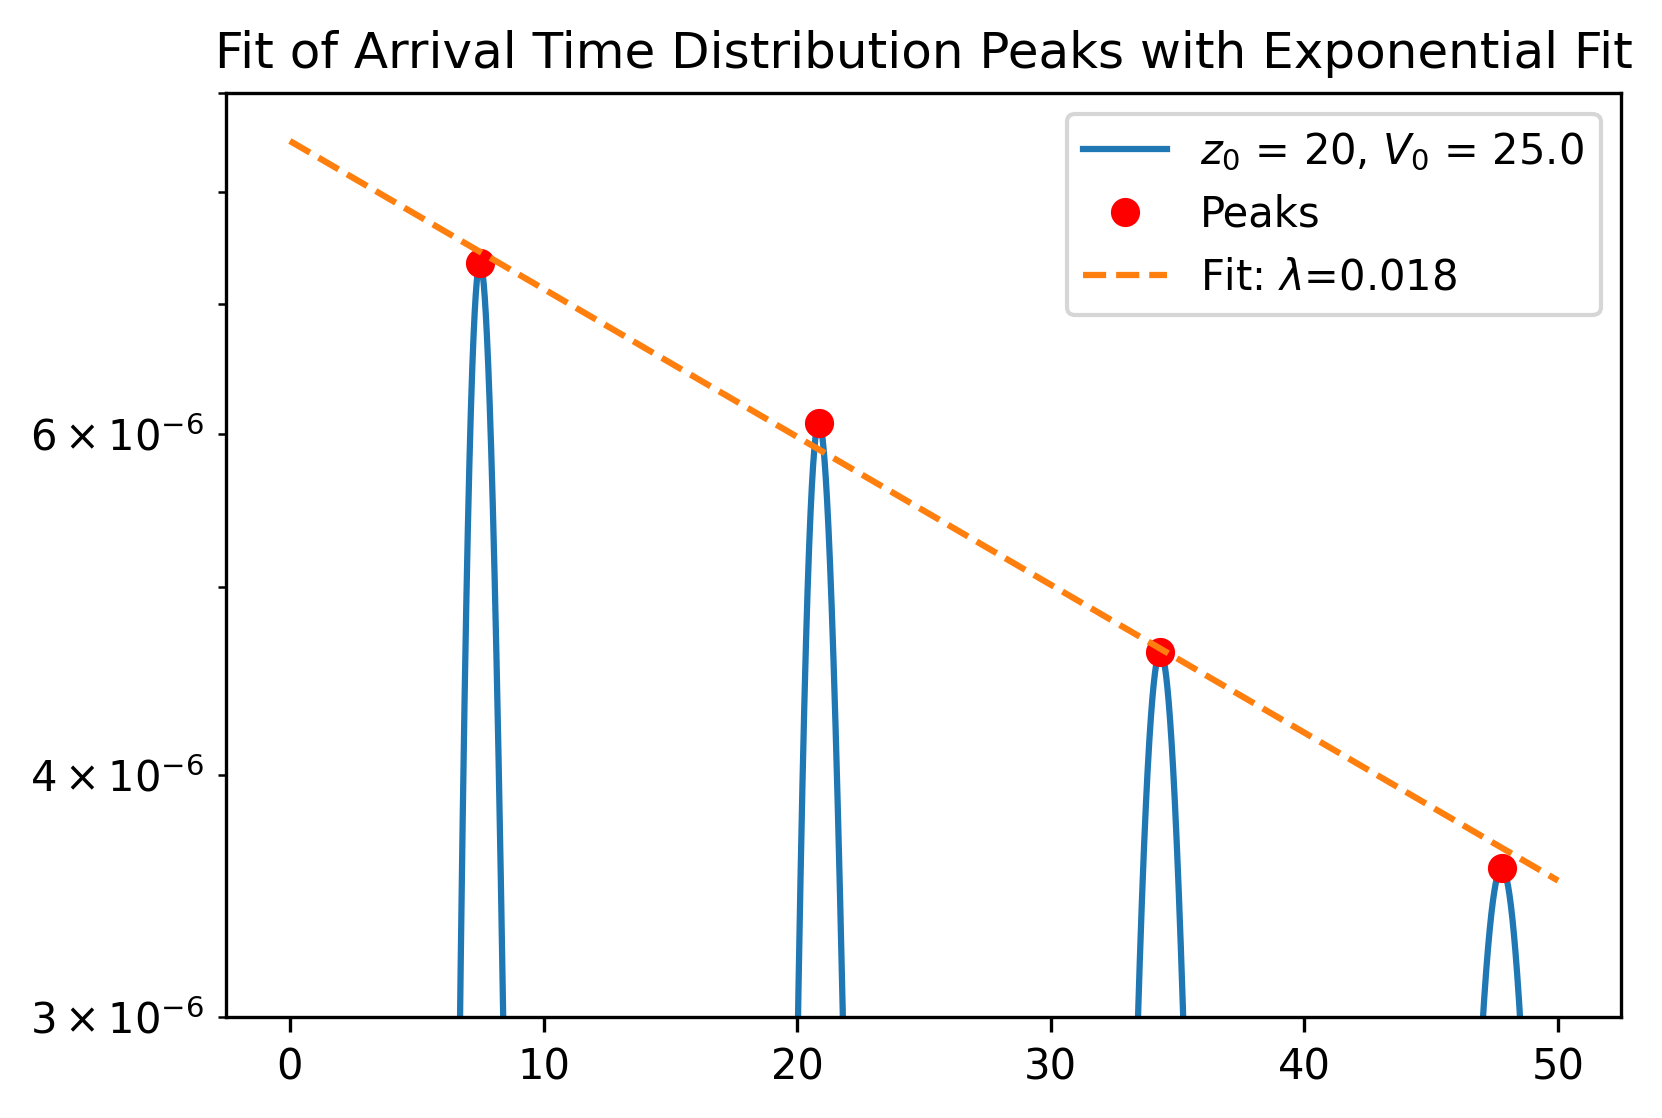
\includegraphics[width=1\linewidth]{Figures//Yoshida/7d9ebeb9-8c0c-45c8-a44b-739e39178c7e.png}
    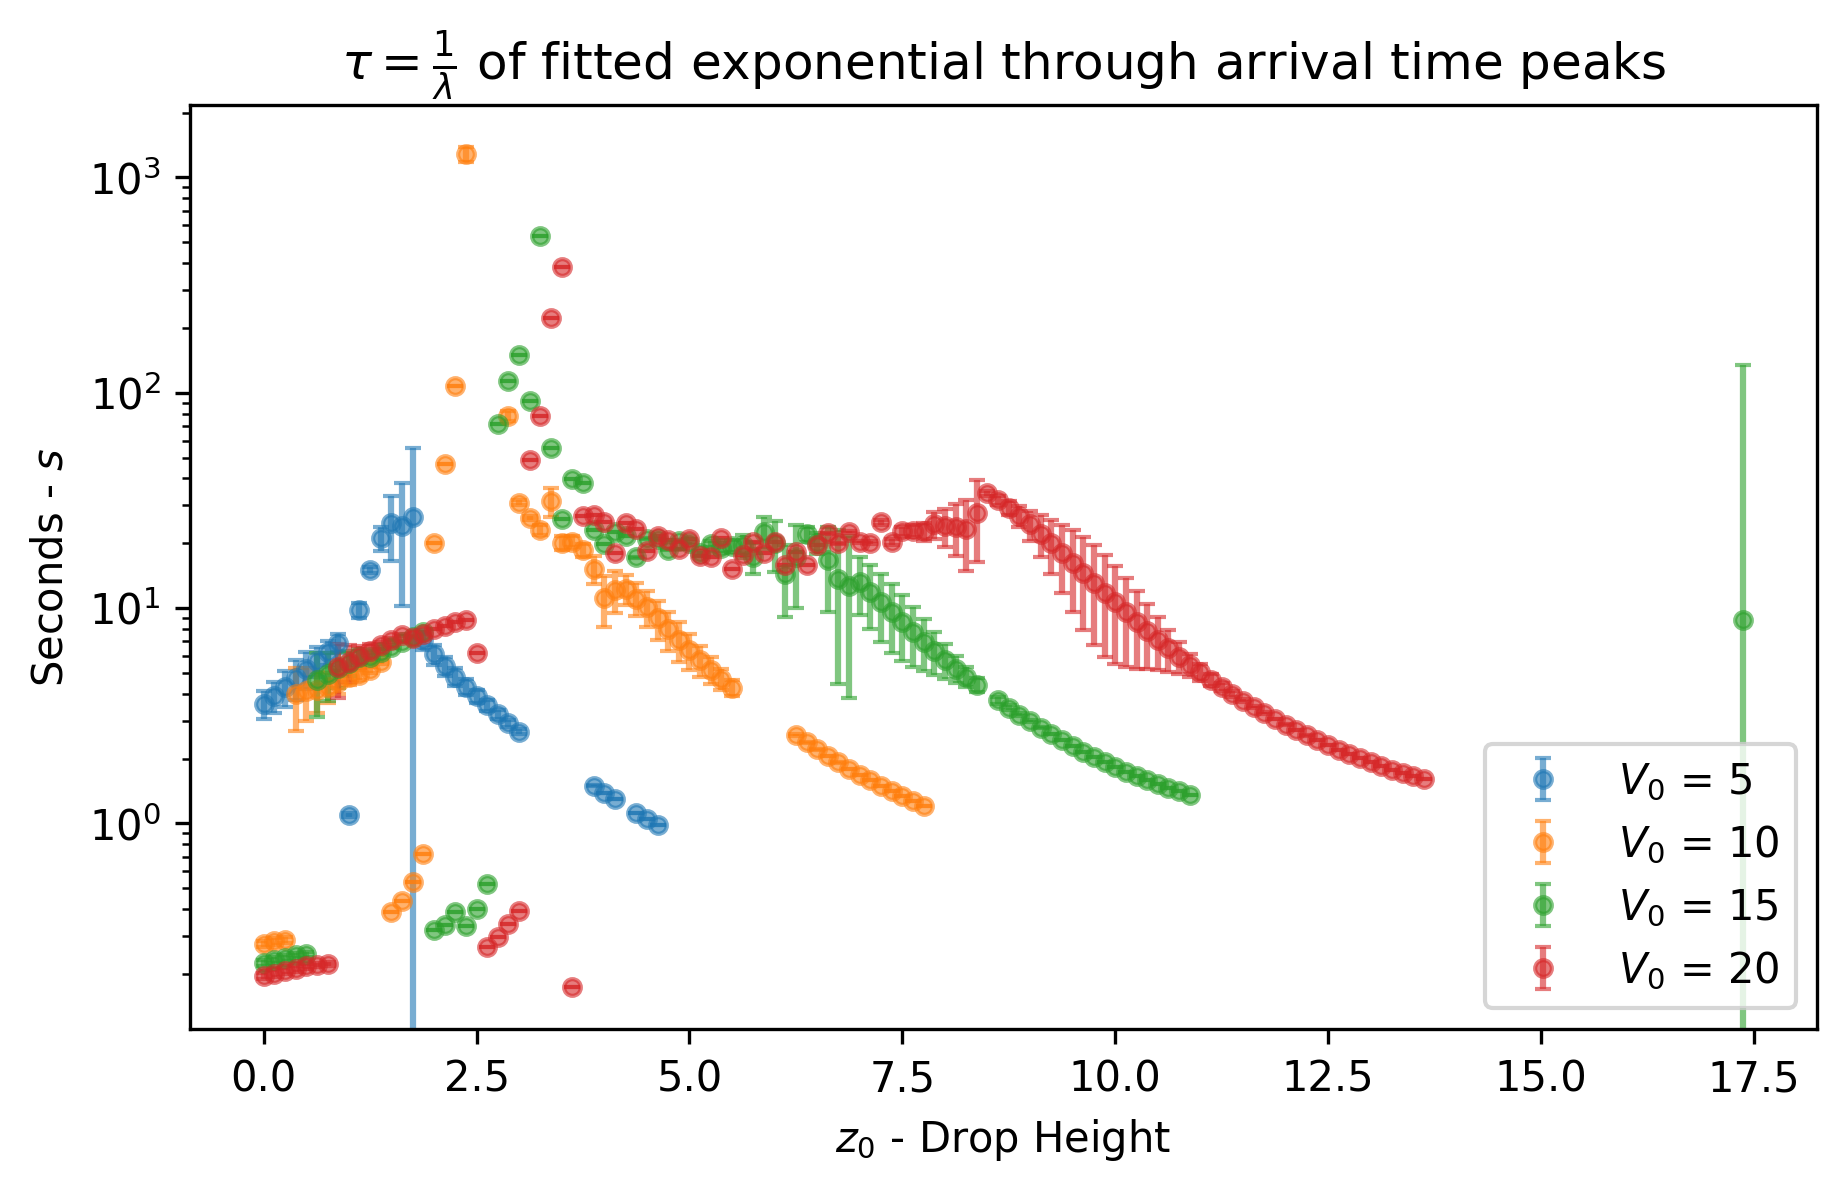
\includegraphics[width=1\linewidth]{Figures//Yoshida/0c0a8ea4-42db-4ad1-b609-e2cd504f8f1d.png}

    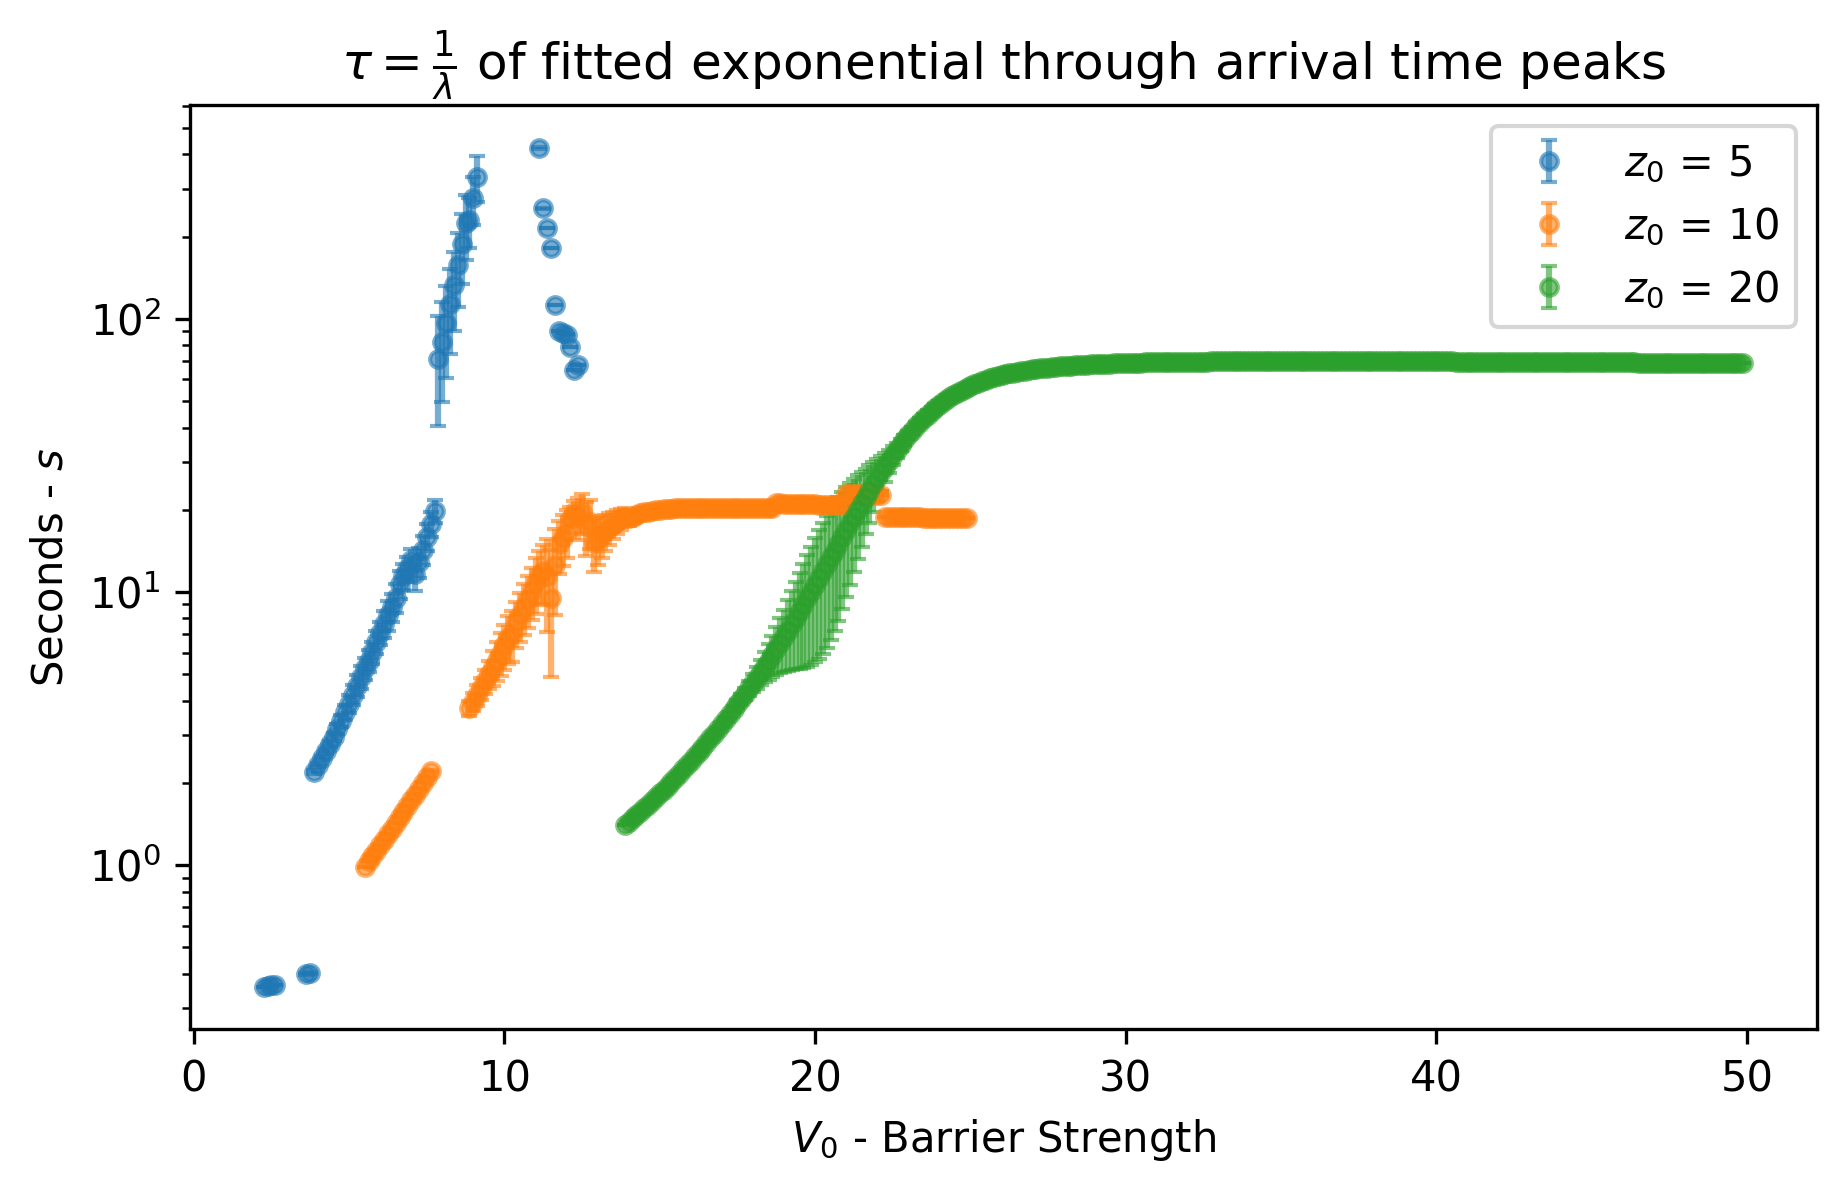
\includegraphics[width=1\linewidth]{Figures//Yoshida/e5c951e3-0e44-432a-b02f-c071aa8b88d5.png}
    \caption{Value of fitted parameter $\tau = \frac{1}{\lambda}$ through arrival time peaks. Error bars represent mean square error times a constant factor 3000 to make them visible. The figure on top has units "Barrier Strength" on the x-axis, and "PPT" - Probability Per Unit Time on the y-axis. Missing $\tau$ values are indicative of no adequate fits, or absence of enough peaks (3) for fitting to proceed.}
    \label{fig:peak_barrier_vs_j}
\end{figure}


\subsection{Tunnelling Time - Bohmian vs Larmor Clocks}

With over 400 $\times$ 2D simulations conducted, the tunnelling time using Bohmian trajectories and Larmor Clock Theory seem to coincide in the weak field regime, for circular barriers: $\tau_{\text{larmor}} = 0.172 \pm1.51\times10^{-6}$ and $\tau_{\text{bohm}} = 0.170 \pm2.77\times10^{-17}$ across the considered weak field range and setup parameters.

\begin{figure}
    \centering
    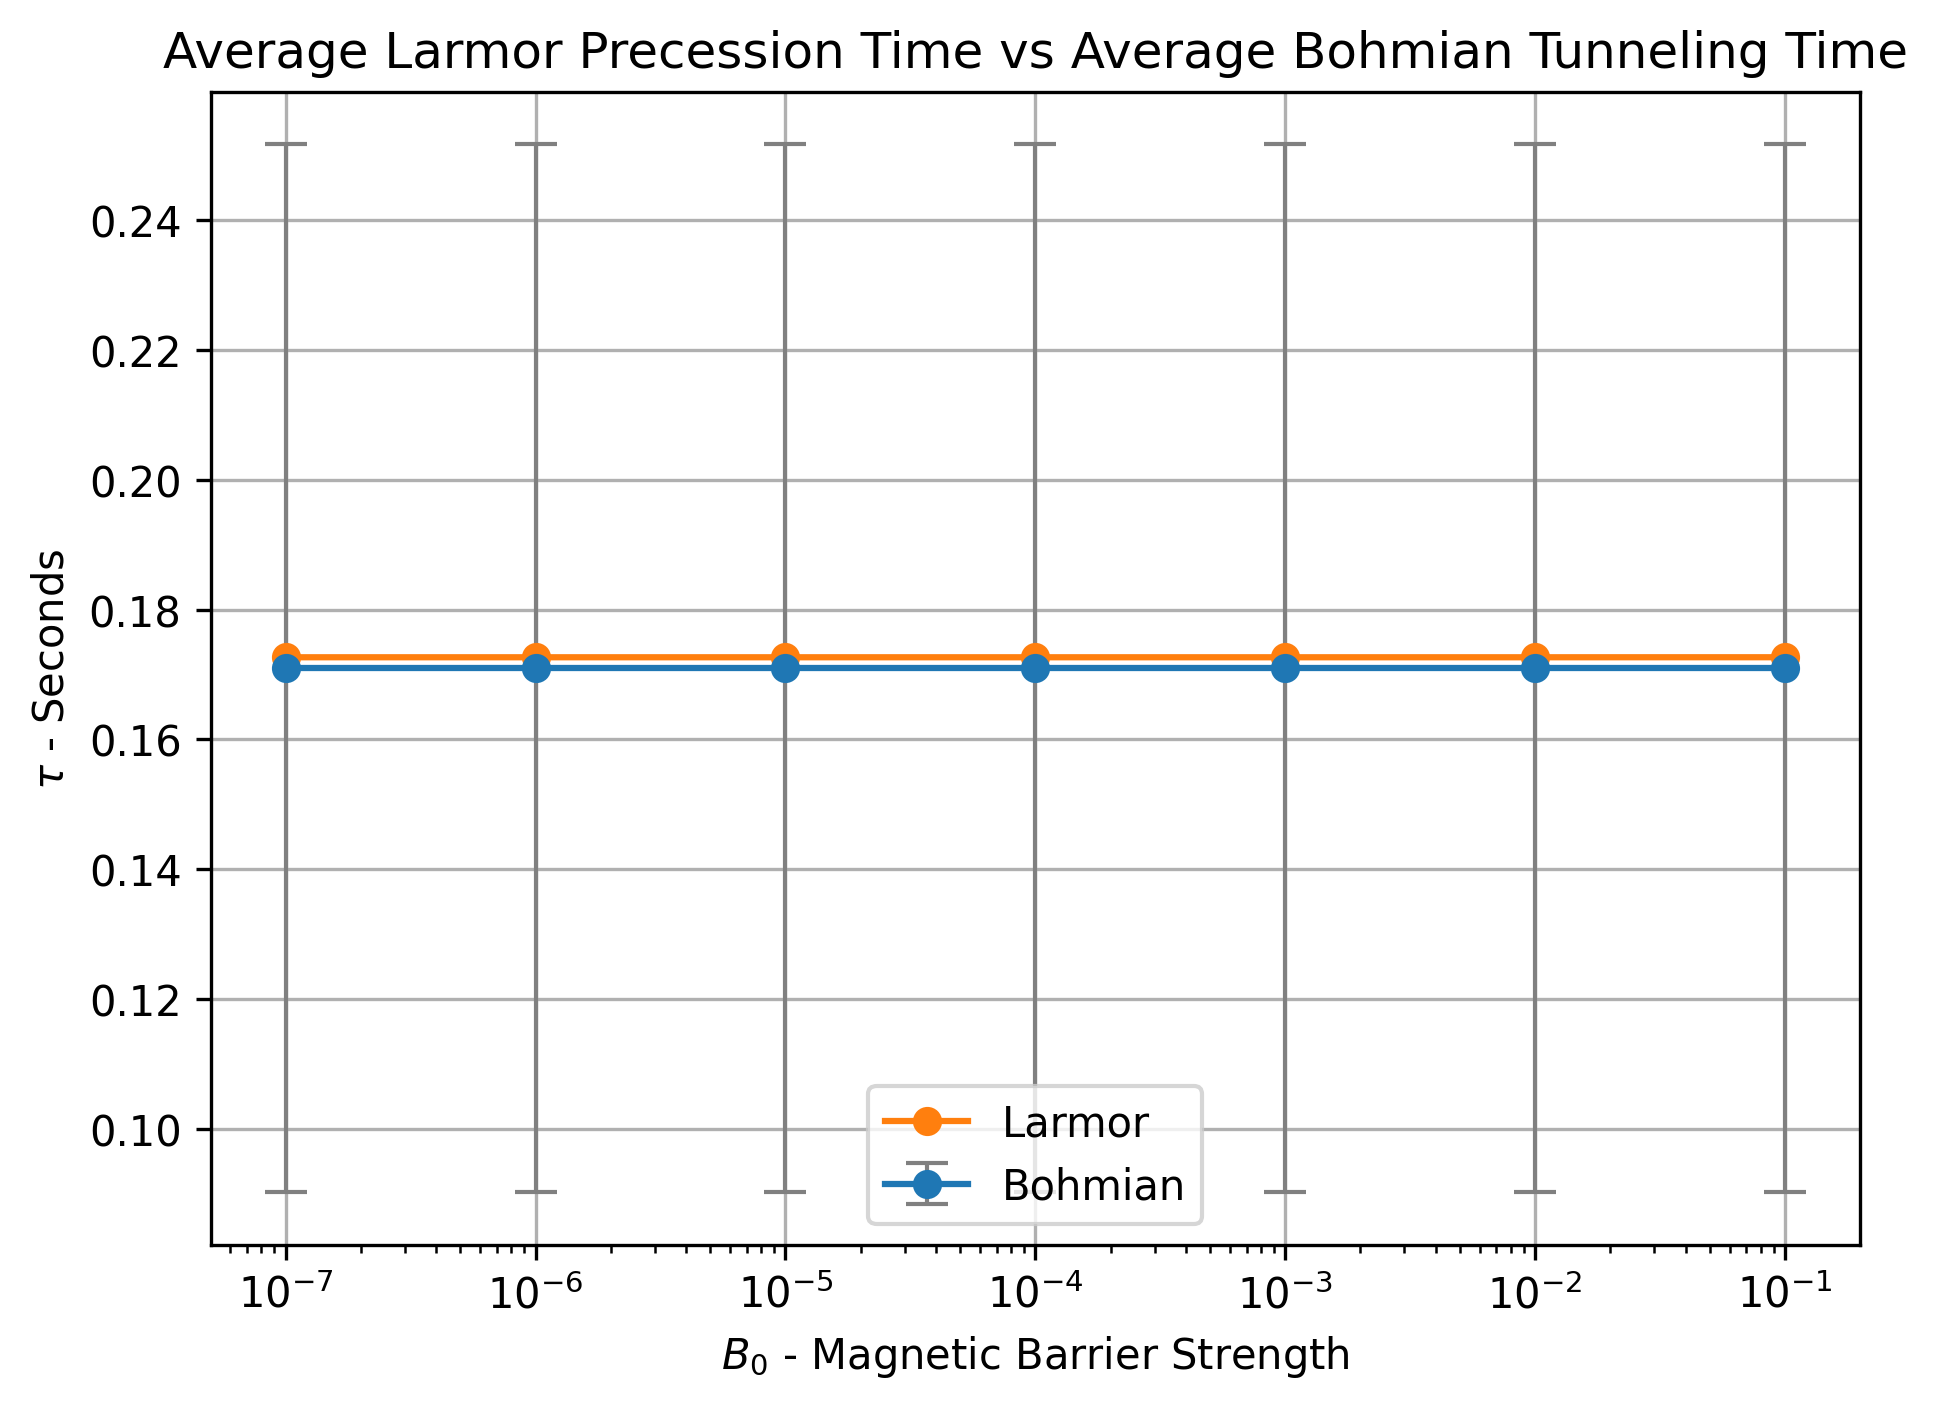
\includegraphics[width=1\linewidth]{Figures//2dspin/353e2f92-95a8-4c1b-b7b5-79fe511d7af9.png}
    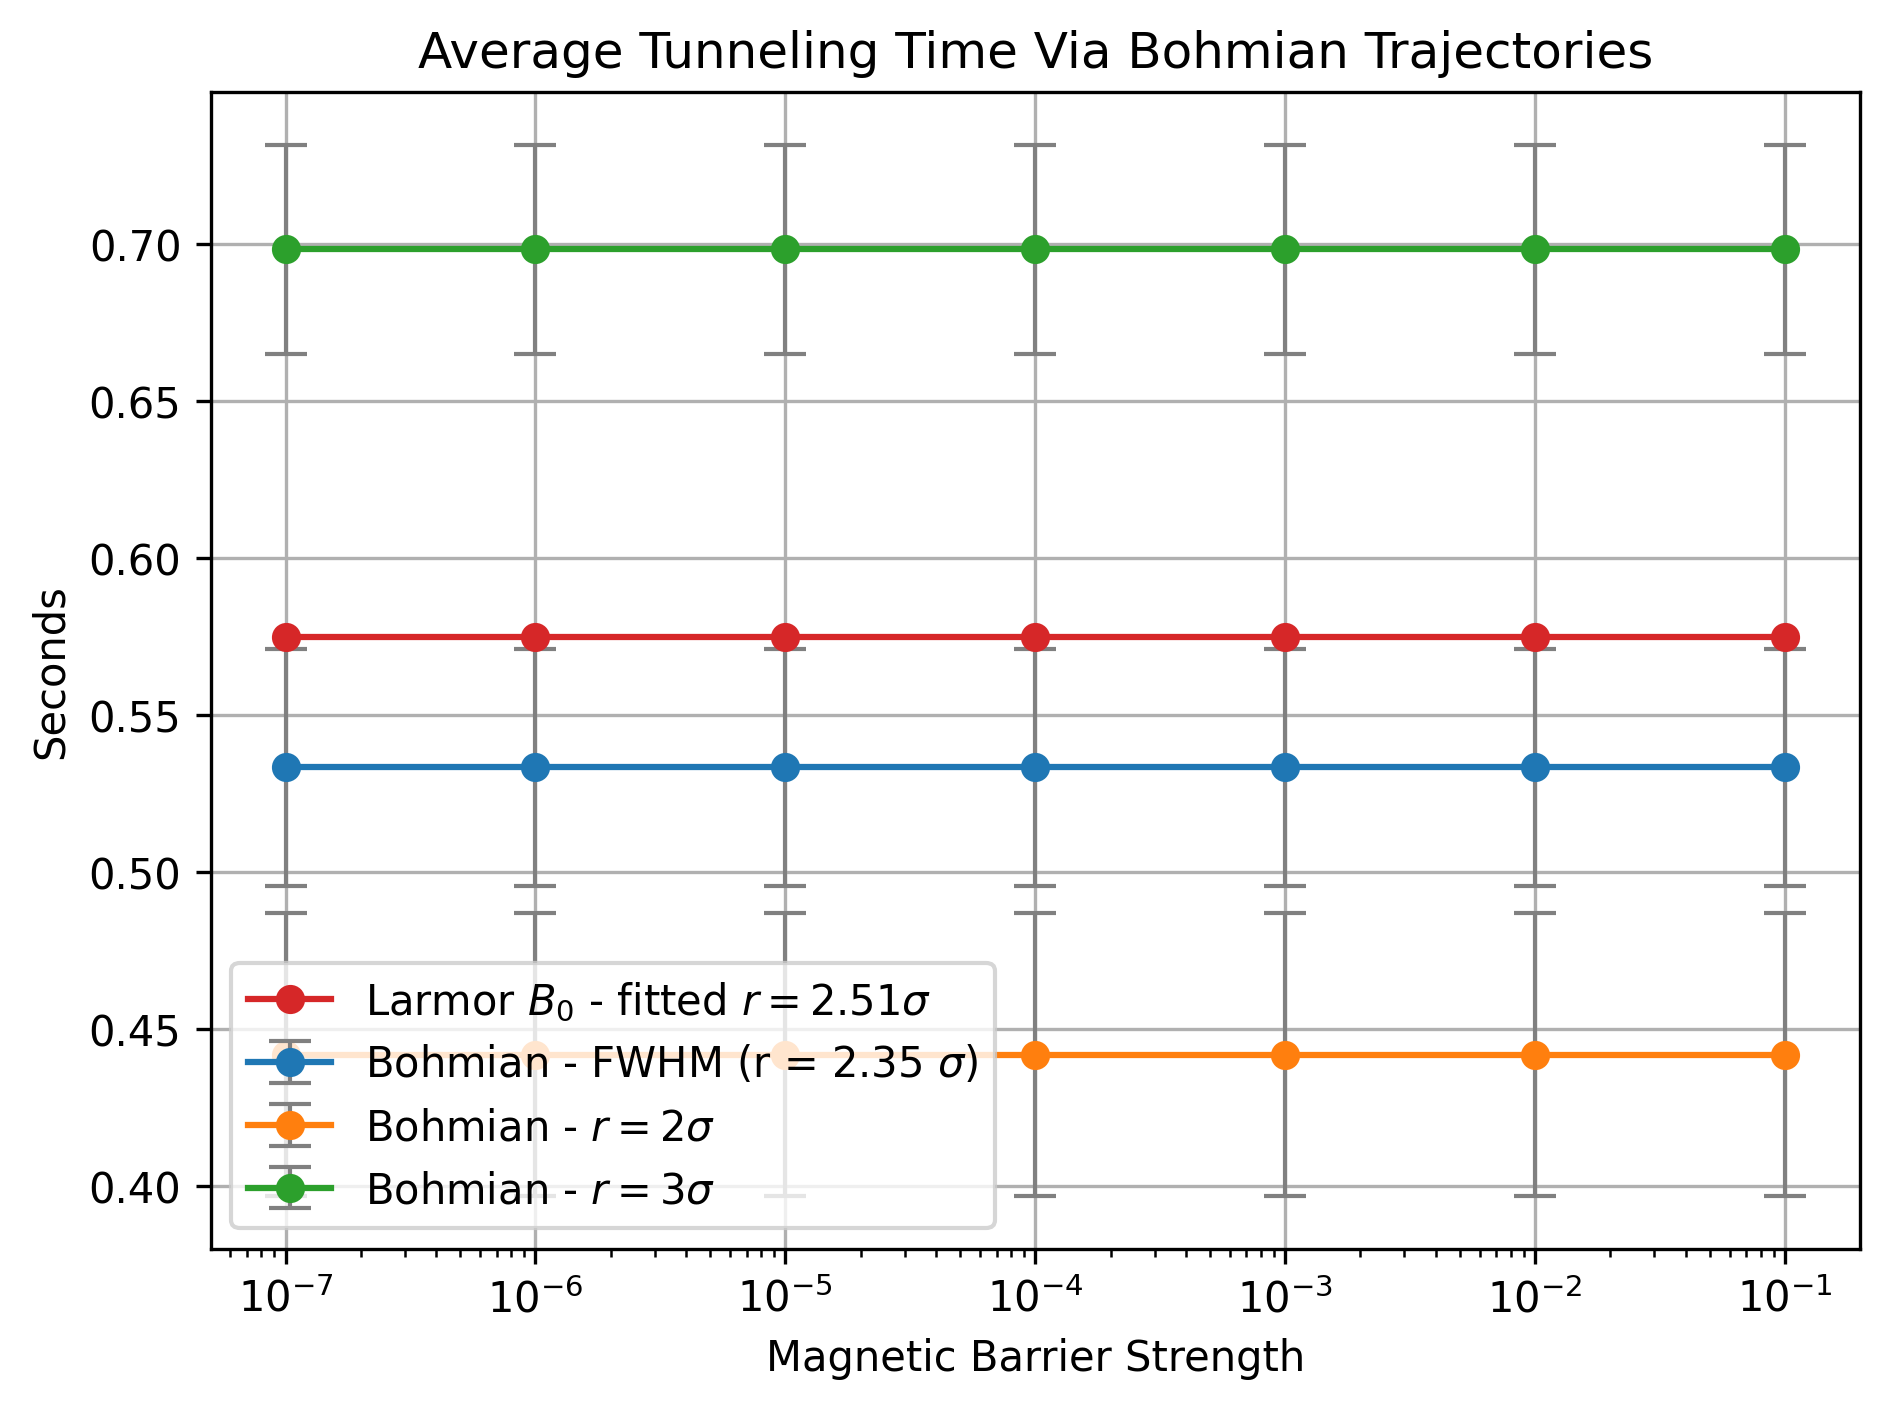
\includegraphics[width=1\linewidth]{Figures//2dspin/70557699-091f-4e39-a011-df61dbb7382d.png}
    
    \caption{Tunnelling Times For a Circular Uniform Barrier with a clear boundary (a), and a Gaussian barrier (b) both using Larmor Precession Times $\tau_L$, and Bohmian trajectories. These data points are obtained in the weak field regime. At low magnetic strengths, the two seem to coincide. Error bars on the Bohmian tunnelling time represent 1 standard deviation over the average Bohmian trajectory ensemble.}
    \label{fig:tunneling_times}
\end{figure}

Bohmian Tunnelling time for Gaussian barriers seems to be problematic, mainly because it has no well-defined boundary, making boundary choice arbitrary. The Larmor Clock read $\tau = 0.574 \pm 7.81\times10^{-8} s$ across the weak field region. The tunnelling times are plotted against one other in figure \ref{fig:tunneling_times} with strong field simulations and tunnelling time results available in the appendix on page \pagref{fig:abc67rtyfugiop}. To make the Bohmian trajectories coincide with Larmor clock time, the width of the boundary for counting Bohmian trajectories ought to be considered at $2R=2.51 \sigma$, which is just a little bit wider than the FWHM of a Gaussian, the experimentalist's definition of a typical laser width. This value was fitted using basic numeric iterations.